\chapter{Results}

The results are retrieved running simulations based on the previous chapters. The different parameters are defined in detail in Appendix B.

Every simulation is run ten times and the mean and standard deviation($\sigma$) are calculated. The source code for the simulation is available online~\cite{repository:me:thesis} . The settings used to generate these particular results is also available in the preset directory. 

%For the most part, most environment variables are not mentioned as they affect the strategies the same. 

\section{Fee Price}

A probabilistic fee model, as suggested in Section \ref{probabilistic}, was generated by running three sequential simulation cycles. A simulation was then set up with half the initial nodes using the generated fee model, while the other half used an uniform random model. The fee model clearly outperforms the random model as seen in Figure \ref{fig:history_price}. The results also shows that the fee is more crucial than the attachment strategy. 

\begin{figure}[!htb]

	\hspace*{-0.5cm}\ 
	\centering
	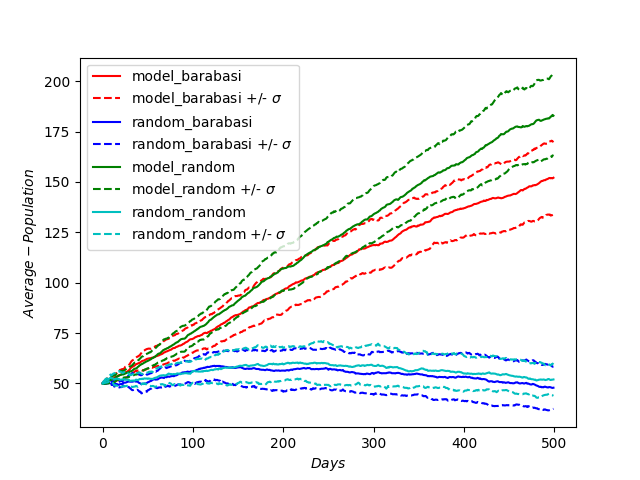
\includegraphics[width=9cm]{images/histories_deviation_price.png}
	\caption{ The history of the node count averages with one standard deviation, for 10 runs. Initially half of the nodes utilizing the generated fee model and the other half a random model. Similarly the attachment strategies are split between Random and Barabasi-Albert. All other strategies are kept equal.
	}
	\label{fig:history_price}
	\hspace*{2mm} 
\end{figure}

\section{Attachment}

The different attachment strategies, excluding biases, were simulated against each other. The results is seen in Figure \ref{fig:history_attachment} 

\begin{figure}[!htb]
	
	\hspace*{-0.5cm}
	\centering
	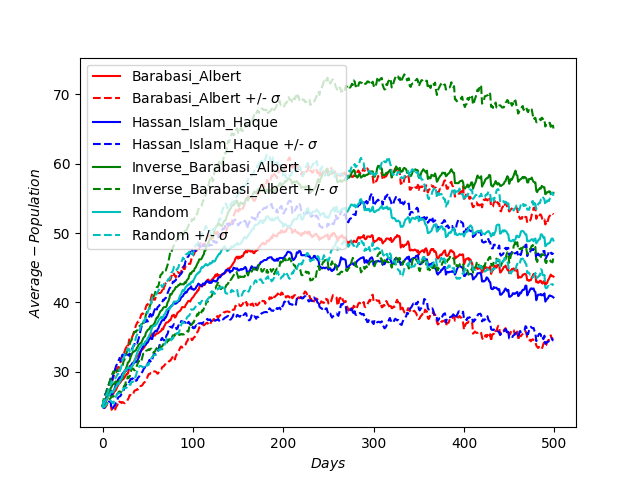
\includegraphics[width=9cm]{images/histories_deviation_attachment.png}
	\caption{ Shows the node count average with one standard deviation for four attachment strategies, Random, Barabasi-Albert, Hassan-Islam-Haque and Inverse-Barabasi for. All else being equal. }
	\label{fig:history_attachment}
	\hspace*{2mm} 
\end{figure}

\section{Funding}

A simulation with four different level of funding was simulated. Each increasing step had twice the funding. The results seen in Figure \ref{fig:funding} suggests that it may be advantageous to be an outlier. Since allocation per channel is equal, this essentially hints at difference in amounts of open channels.

\begin{figure}[!htb]
	%\hspace*{-1cm}\
	\centering
	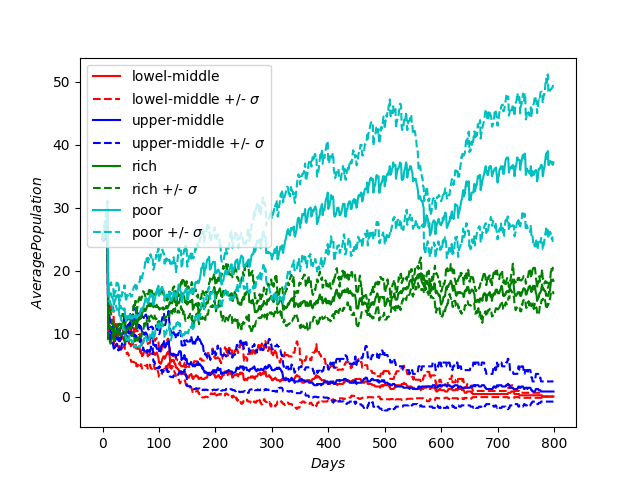
\includegraphics[width=9cm]{images/histories_deviation_fund.png}
	\caption{ Displays the node count and node count average with one standard deviation for four different levels of funding. All other strategies being equal.
	}
	\label{fig:funding}
	\hspace*{2mm} 
\end{figure}


(preferential attachment)

(funding)

(open close)

(degree distribution)
(profit distribution)

(re-balance channel)

(combined best strategies)

(is strategy set stable from invasion)

(external pressures, payment pressure, routing / private channels.)